\iffalse
\documentclass[journal,12pt,twocolumn]{IEEEtran}
\usepackage{amsmath,amsfonts,amssymb,float,gvv,graphicx,enumitem,array,esint}
\bibliographystyle{IEEEtran}
\vspace{3cm}
\title{GATE 2023-ME-50}
\author{Pragnidhved Reddy\\EE23BTECH11050}
\date{}
\parindent 0px
\begin{document}
\maketitle
\newpage
\bigskip
\textbf{Question GATE 23 ME 50:}\\
The initial value problem
$\frac{dy}{dt}+2y=0, y(0)=1 $
is solved numerically using the forward Euler's method with a constant and positive time step of $\delta $.\\
Let $y_n$ represent the numerical solution obtained after $n$ steps. The condition $\abs{y_{n+1}} \leq \abs{y_n}$is satisfied if and only if $\delta$ does not exceed\\
\solution \\
\fi
Numerical solution: -\\
By forward Euler's method formula 
\begin{align}
\label{eq:eq1_ME_50}
    y(n+1)=y(n)+\delta  f(x,y)
\end{align}
From question we get
\begin{align}
\label{eq:eq2_ME_50}
\frac{dy}{dx}=-2y=f(x,y)
\end{align}
From \eqref{eq:eq2_ME_50} in \eqref{eq:eq1_ME_50}
\begin{align}
y(n+1)-y(n)&=-2\delta y(n)\\
y(n+1)&=(1-2\delta)y(n)\\
y(n)&\overset{Z}\longleftrightarrow Y(z)\\
y(n+1)&\overset{Z}\longleftrightarrow zY(z)-y(0)\\
\implies zY(z)-y(0)&=(1-2\delta)Y(z)\\
Y(z)&=\frac{1}{z-1+2\delta}\\
\frac{1}{z-(1-2\delta)}&\overset{Z}\longleftrightarrow (1-2\delta)^{n}u(n)
\end{align}
For good approximation we choose $\delta$ = 0.4
\begin{align}
y(n)&=(0.2)^nu(n)
\end{align}
Now using the condition given in question
\begin{align}
|y(n+1)| \leq |y(n)|\\
|(1-2\delta)^2| \leq |1-2\delta|\\
|1-2\delta| \leq 1 \\
0 \leq \delta \leq 1
\end{align}
From this we can say that the maximum value of $\delta  $ is 1\\
Theoritical solution: -\\
By properties of Laplace transform: -
\begin{align}
\label{eq:eq8_ME_50}
Y(s)&=\mathcal{L}y(s)\\
\label{eq:eq9_ME_50}
\mathcal{L}y'&=sY(s)-y(0)
\end{align}
Given equation: -
\begin{align}
y'+2y&=0\\
\mathcal{L}(y'+2y)&=0
\end{align}
From \eqref{eq:eq8_ME_50} and \eqref{eq:eq9_ME_50}
\begin{align}
sY(s)-1+2Y(s)&=0\\
\frac{1}{s+2}&=Y(s)\\
y(t)&=\mathcal{L}^{-1}Y(s)\\
\implies y(t)&=\mathcal{L}^{-1}\left(\frac{1}{s+2}\right)\\
\mathcal{L}^{-1}\left(\frac{1}{s+k}\right)&=e^{-kt}u(t)\\
\implies y(t)&=e^{-2t}u(t) 
\end{align}
\begin{figure}[h!]
    \centering
    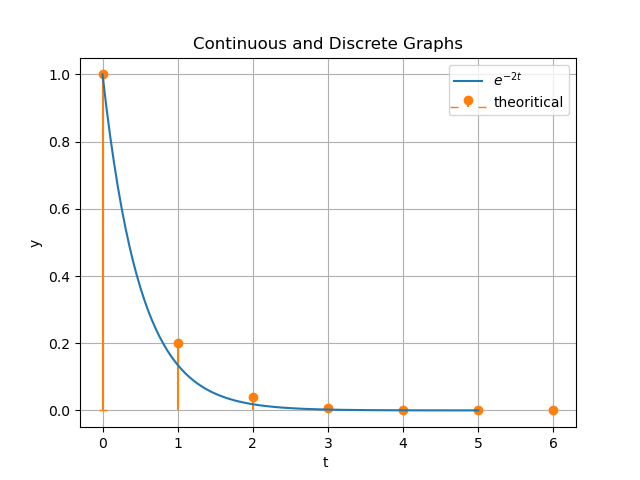
\includegraphics[width=\columnwidth]{2023/ME/50/figs/graph.png}
    \caption{simulation vs analysis}
\end{figure}


